\begin{figure}[H]
    \centering

    \begin{subfigure}[t]{.3\textwidth}
        \centering
        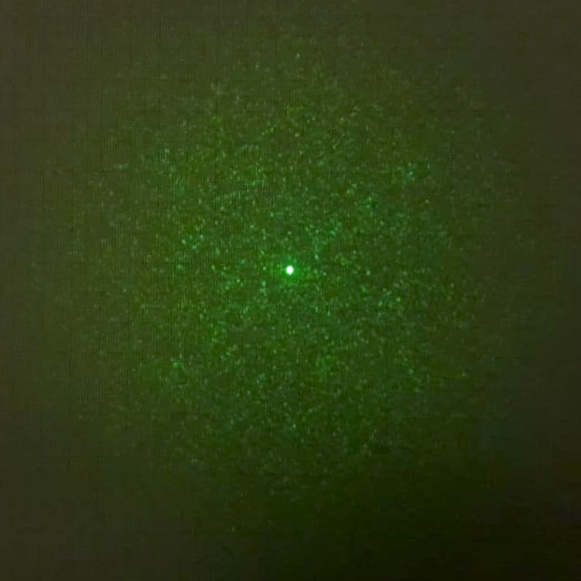
\includegraphics[width=\textwidth]{figuras/medidas/D1.jpg}
        \caption{D1}
        \label{fig:D1}
    \end{subfigure}
    \qquad
    \begin{subfigure}[t]{.3\textwidth}
        \centering
        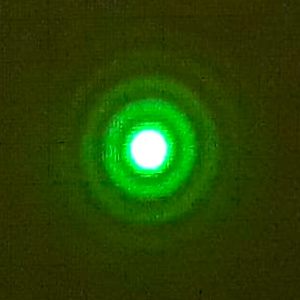
\includegraphics[width=\textwidth]{figuras/medidas/D2.jpg}
        \caption{D2}
        \label{fig:D2}
    \end{subfigure}
    \qquad
    \begin{subfigure}[t]{.3\textwidth}
        \centering
        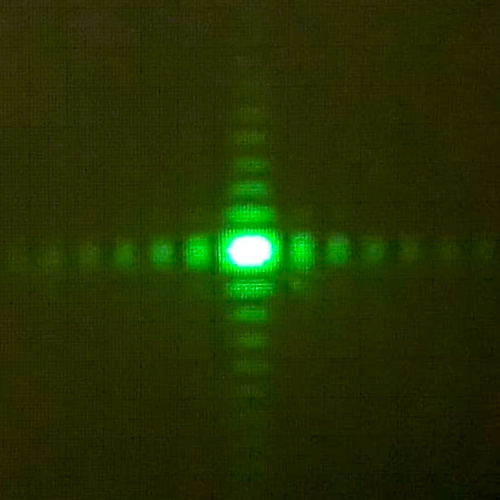
\includegraphics[width=\textwidth]{figuras/medidas/D3.jpg}
        \caption{D3}
        \label{fig:D3}
    \end{subfigure}
    \qquad
    \begin{subfigure}[t]{.3\textwidth}
        \centering
        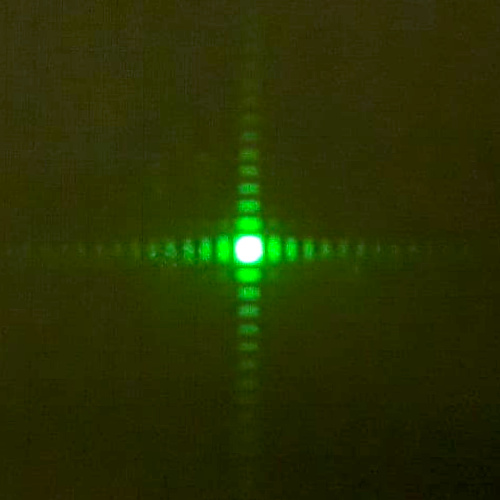
\includegraphics[width=\textwidth]{figuras/medidas/D4.jpg}
        \caption{D4}
        \label{fig:D4}
    \end{subfigure}
    \qquad
    \begin{subfigure}[t]{.3\textwidth}
        \centering
        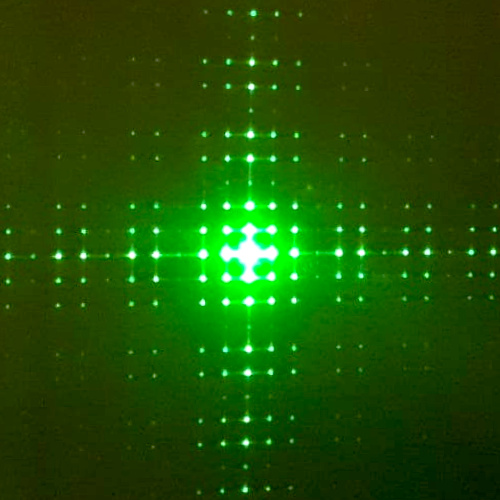
\includegraphics[width=\textwidth]{figuras/medidas/D5.jpg}
        \caption{D5}
        \label{fig:D5}
    \end{subfigure}
    \qquad
    \begin{subfigure}[t]{.3\textwidth}
        \centering
        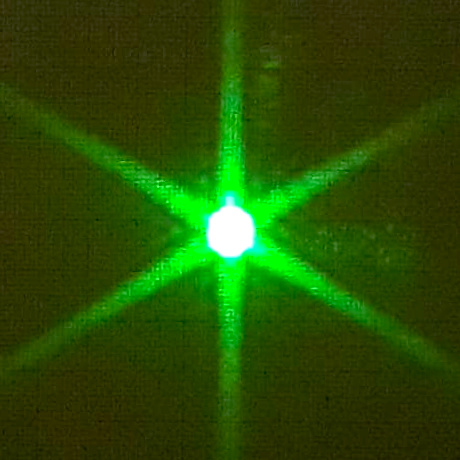
\includegraphics[width=\textwidth]{figuras/medidas/D6.jpg}
        \caption{D6}
        \label{fig:D6}
    \end{subfigure}

    \caption{Fotos dos padrões de difração das fendas D}
    \label{fig:D}
\end{figure}